\documentclass[aspectratio=169]{beamer}

\usetheme{default}

\usepackage[utf8]{inputenc}
\usepackage[russian]{babel}
\usepackage[OT1]{fontenc}
\usepackage{amsmath}
\usepackage{amsfonts}
\usepackage{amssymb}
\usepackage{graphicx}
\usepackage{etoolbox}
\usepackage{caption}
\usepackage{subcaption}
\captionsetup{compatibility=false}
\usepackage{pifont}
%\usepackage{subfigure}
\usepackage{xcolor}
\usepackage{framed}
\usepackage{empheq}
\usepackage[many]{tcolorbox}
\usepackage{multirow}
\usepackage{tikz}
\usepackage{listings}
\usepackage{tikz}

\definecolor{shadecolor}{cmyk}{0,0,0,1}

\lstset{
	backgroundcolor=\color{lightgray},
	commentstyle=\color{blue},
	frame=single
	breakatwhitespace, 
	language=python, 
	columns=fullflexible, 
	keepspaces, 
	breaklines, 
	tabsize=3, 
	showstringspaces=false, 
	extendedchars=true,
	numbers=left
}

\makeatletter

\setbeamercolor{title}{fg=white}
\setbeamercolor{frametitle}{fg=black}
\setbeamerfont*{title}{family=\sffamily,size=\LARGE}

\setbeamerfont{page number in head/foot}{size=\scriptsize}
\setbeamertemplate{footline}[frame number]
\let\otp\titlepage
\renewcommand{\titlepage}{\otp\addtocounter{framenumber}{-1}}

\setbeamertemplate{background canvas}{%
	\ifnumequal{\c@framenumber}{0}{%
		\vbox to \paperheight{\vfil\hbox to \paperwidth{\hfil
\includegraphics[height=\paperheight]{images/cover.png}\hfil}\vfil}
   }{%
      \ifnumequal{\c@framenumber}{\inserttotalframenumber}{
        \vbox to \paperheight{\vfil\hbox to \paperwidth{\hfil
\includegraphics[height=\paperheight]{images/back.png}\hfil}\vfil}
      }{%
         % Other frames
      }%
   }%
}

\makeatother

\beamertemplatenavigationsymbolsempty

\tcbset{highlight math style={enhanced,colframe=red,colback=white,arc=4pt,boxrule=1pt}}

\usetikzlibrary{shadings,shadows,shapes.arrows}

\newcommand*{\tikzarrow}[2]{%
  \tikz[
    baseline=(A.base),             % Set baseline to the baseline of node content
    font=\footnotesize\sffamily    % Set fontsize of the node content
  ]
  \node[
    single arrow,                  % Shape of the node
    single arrow head extend=5pt,  % Actual width of arrow head
    draw,                          % Draw the node shape
    inner sep=3pt,                 % Separation between node content and node shape
    top color=#1,               % Shading color on top of node
    bottom color=#1,               % Shading color on bottom of node
    % drop shadow                    % Draw a shadow
  ] (A) {#2};%
}

\newcommand{\tikzfancyarrow}[2][2cm]{\tikz[baseline=-0.5ex]\node [arrowstyle=#1] {#2};}
\newcommand*\rot{\rotatebox{90}}

\author{Николай Анохин}
\title{\newline \newline \newline Лекция 11 \\ Data Mining в реальных системах}

\begin{document}

\begin{frame}[plain]
\titlepage
\end{frame}

\begin{frame}{}

\begin{center}
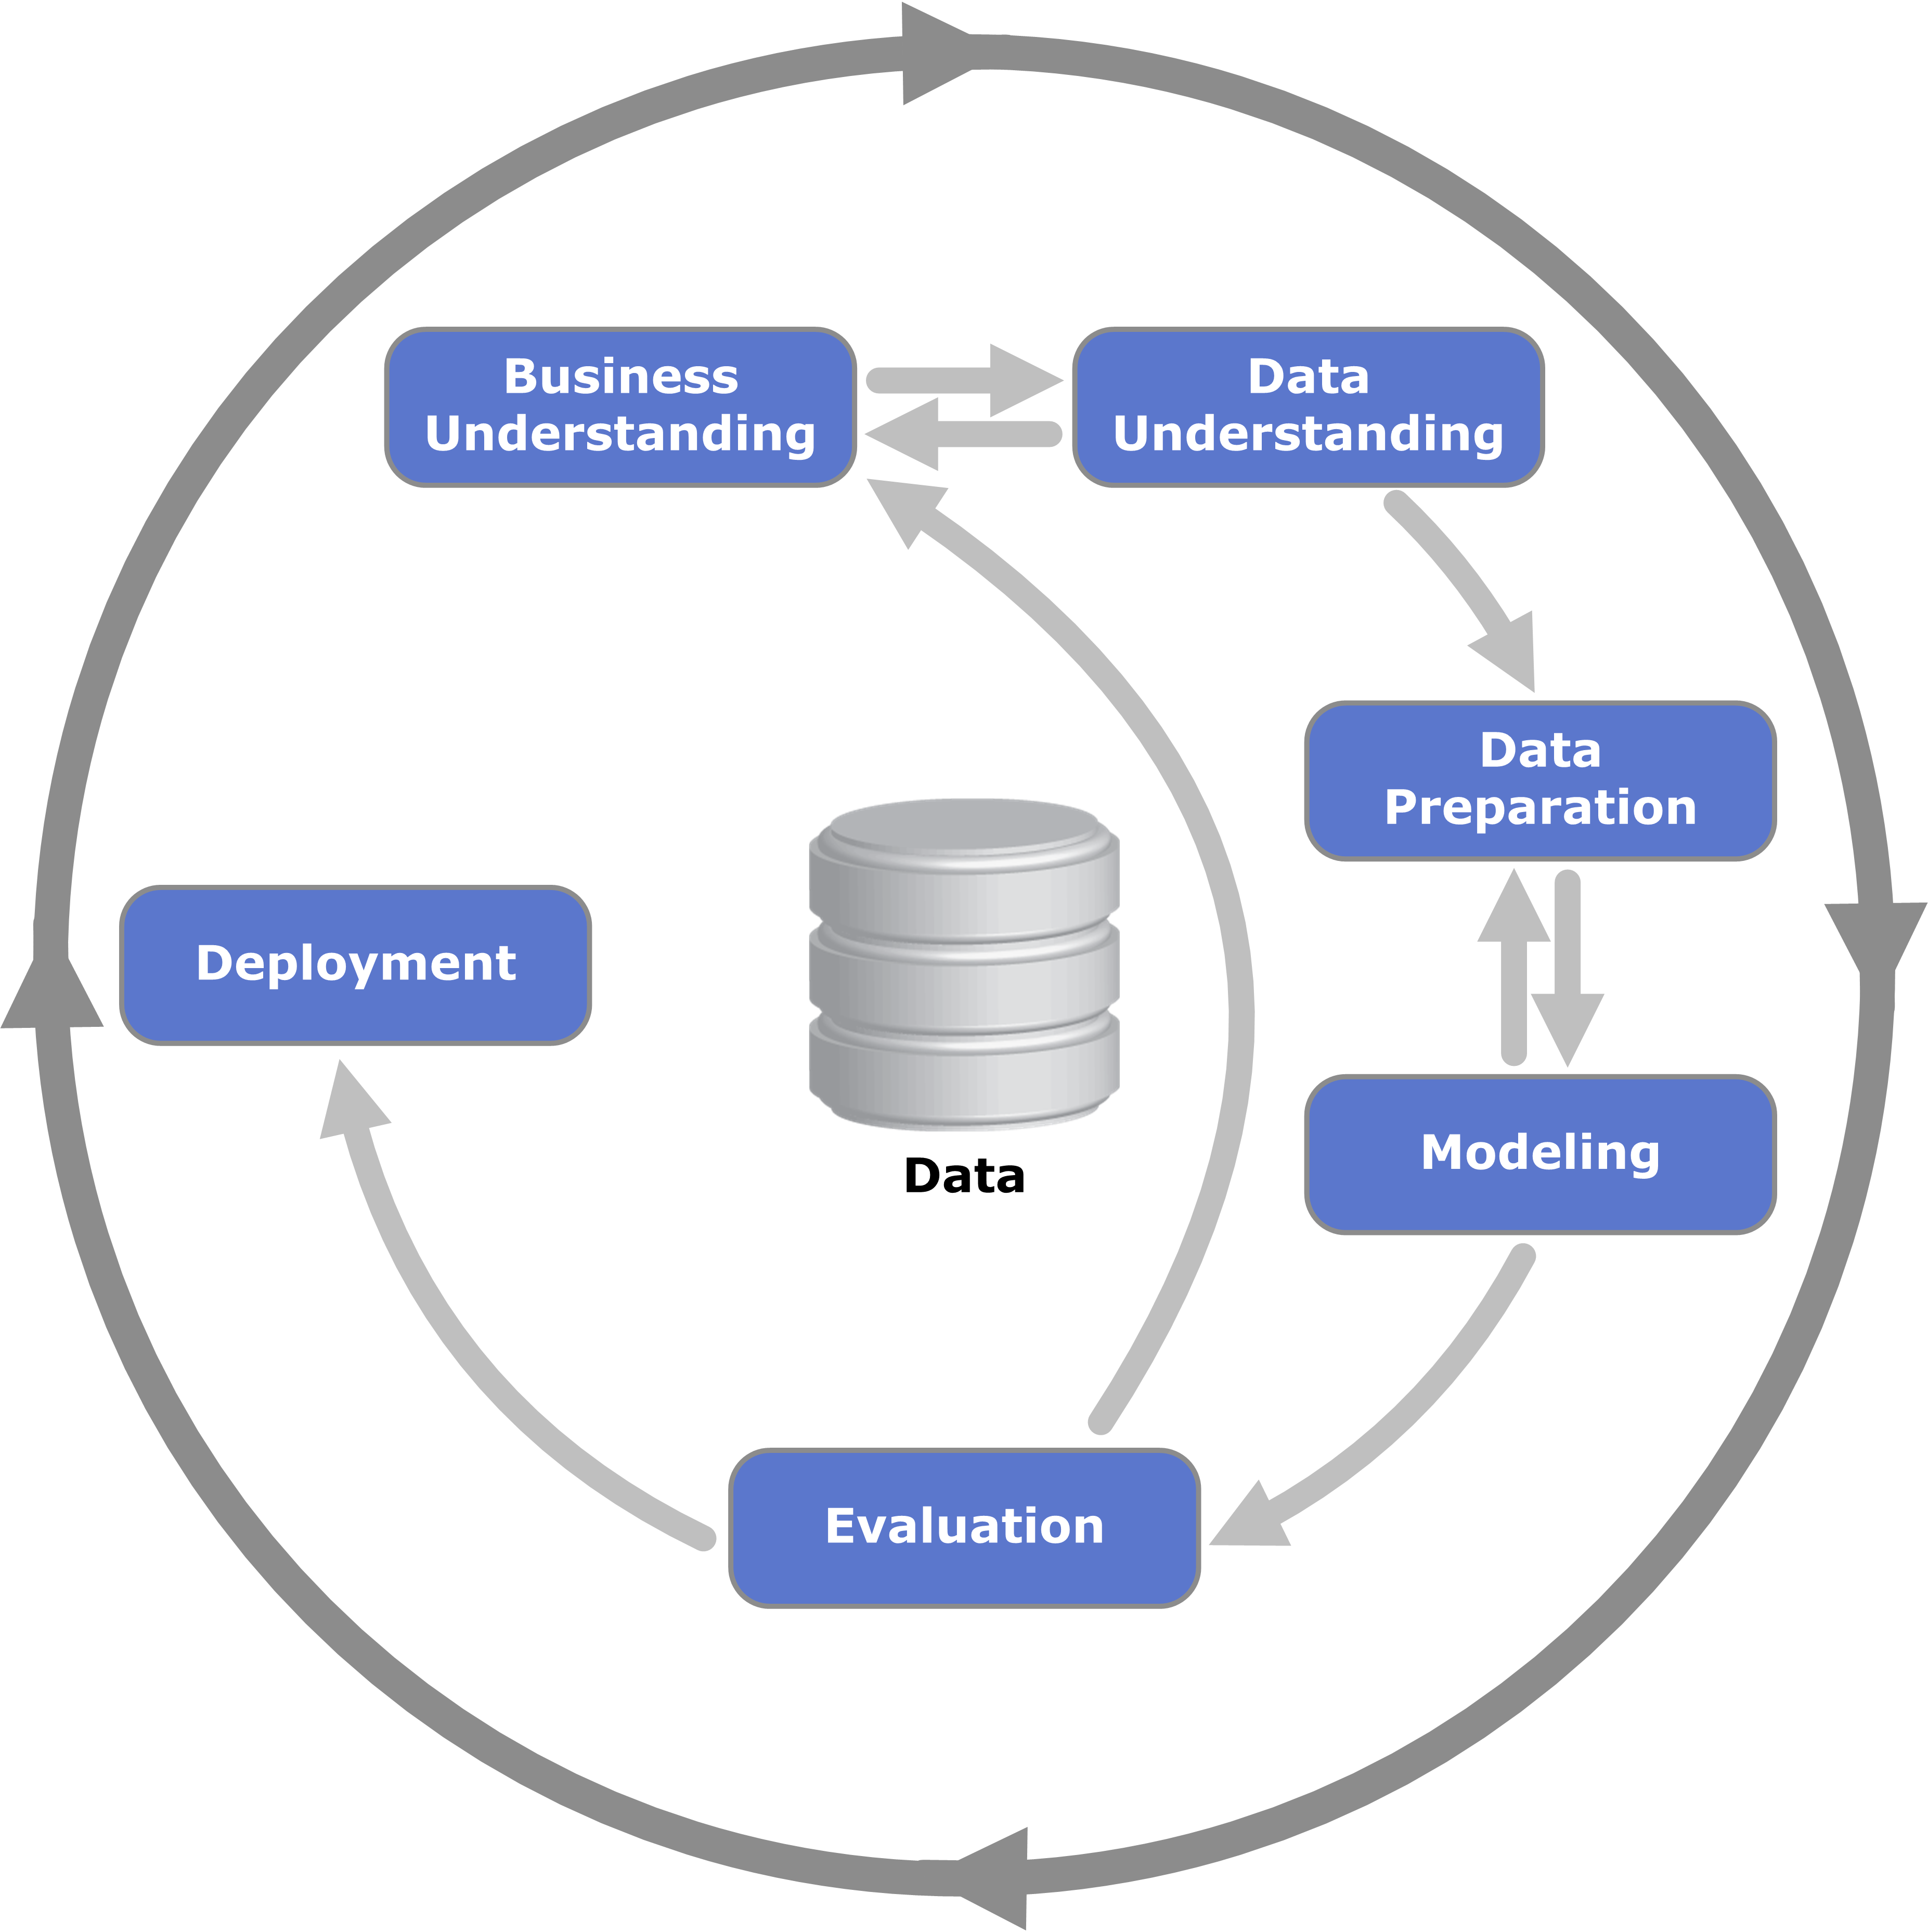
\includegraphics[scale=0.4]{images/crisp.png}
\end{center}

\end{frame}

\begin{frame}{План занятия}
\tableofcontents
\end{frame}

% ============================================== %

\section{Работа с признаками}

% ============================================== %

\begin{frame}{}

\begin{center}
\Large Работа с признаками
\end{center}

\end{frame}

\begin{frame}[fragile]{Конструирование признаков}

Лог посещения пользователями Интернет-сайтов
\begin{verbatim}
1432068600.002494
46.148.52.217
22B695259
22/159/5/0/0/6/1/1.000000/16.0
2579437
http://vk.com/ivan_se
http://vk.com/friends?act=find
1152*864 
1137*747
1432068601241
Поиск друзей
\end{verbatim}

\end{frame}

\begin{frame}[fragile]{Преобразование признаков}

\begin{itemize}
\item Дискретизация
\item Проекции
	\begin{itemize}
	\item PCA
	\item Random projections
	\end{itemize}
\item Заполнение отсутствующих значений
\item Удаление шума
\item Преобразование категориальных классов в бинарные
	\begin{itemize}
	\item One-vs-rest
	\item One-vs-one
	\item Error correcting output codes
	\begin{verbatim}
	A: 1 1 1 1 1 1 1
	B: 0 0 0 0 1 1 1
	C: 0 0 1 1 0 0 1
	D: 0 1 0 1 0 1 0
	\end{verbatim}
	\end{itemize}
\end{itemize}

\end{frame}

\begin{frame}{Отбор признаков}

Как ``нерелевантные'', так и ``релевантные'' признаки могут быть вредными

\begin{enumerate}
\item Независимо от алгоритма обучения: backward elimnation, forward selection
	\begin{itemize}	
	\item mutual information	
	\item коэффициент корреляции
	\item линейная модель
	\item генетические алгоритмы
	\end{itemize}
\item С использованием алгоритма обучения \\ (кросс-валидация, hold-out)
\end{enumerate}

\end{frame}

% ============================================== %

\section{Алгоритмы машинного обучения}

% ============================================== %

\begin{frame}{}

\begin{center}
\Large Алгоритмы машинного обучения
\end{center}

\end{frame}

\begin{frame}{Некоторые правила 1}

Первое правило машинного обучения
\begin{quote}
Если нет необходимости, не использовать машинное обучение
\end{quote}

Второе правило машинного обучения\footnote{\href{https://homes.cs.washington.edu/~pedrod/papers/cacm12.pdf}{A Few Useful Things to Know about Machine Learning}}
\begin{quote}
\[
LEARNING =
\]
\[
REPRESENTATION + EVALUATION + OPTIMIZATION
\]
\end{quote}

\end{frame}

\begin{frame}{Некоторые правила 2}

\begin{itemize}
\item Обобщающая способность имеет значение
\item Только данных не достаточно
\item У переобучения много видов
\begin{center}
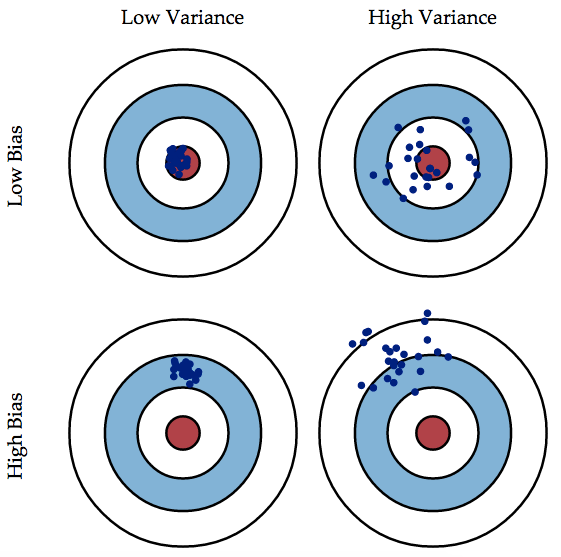
\includegraphics[scale=0.25]{images/bvd.png}
\end{center}
\end{itemize}

\end{frame}

\begin{frame}{Некоторые правила 3}

\begin{itemize}
\item Интуиция подводит в многомерных пространствах
\item Больше данных лучше, чем сложный алгоритм
\item Обучайте много моделей
\begin{center}
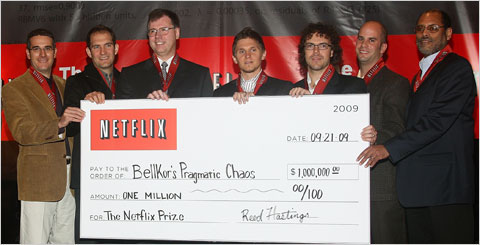
\includegraphics[scale=0.4]{images/netfilx.jpg}
\end{center}
\end{itemize}

\end{frame}

\begin{frame}{Все модели имеют недостатки\footnote{\href{http://web.archive.org/web/20140326142656/http://hunch.net/?p=224}{All Models of Learning have Flaws}}}

\begin{small}
\begin{tabular}{| p{2cm} | p{3.6cm} | p{3.6cm} |}
\hline
Подход & Что хорошо & Что плохо \\
\hline
\hline
bayesian learning & хорошо работает на маленьких данных & трудно обосновать априорные распрделения, вычислительно сложные \\ \hline
градиентный спуск & вычислительно эффективен, оптимизируем что нужно & подбор параметров для сходимости, переобучение \\ \hline
kernel & натуральное выражение схожести через ядро & подбор ядра, медленный \\ \hline
деревья решений & быстрый и автоматизированный & крайне нестабильный \\ \hline
boosting & хорошее качество & выбор алгоритма, предположение о weak learner нарушается  \\
\hline
\end{tabular}
\end{small}

\end{frame}

\begin{frame}{8 худших алгоритмов\footnote{\href{http://www.analyticbridge.com/profiles/blogs/the-8-worst-predictive-modeling-techniques}{The 8 worst predictive modeling techniques}}}

\begin{itemize}
\item Linear regression
\item Traditional decision trees
\item Linear discriminant analysis
\item K-means clustering
\item Neural networks
\item Maximum Likelihood estimation
\item Density estimation in high dimensions
\item Naive Bayes
\end{itemize}

\end{frame}

\begin{frame}{Отбор модели занимает очень много времени\footnote{\href{http://blog.mikiobraun.de/2015/03/three-things-about-data-science.html}{Three Things About Data Science You Won't Find In the Books}}}

\begin{center}
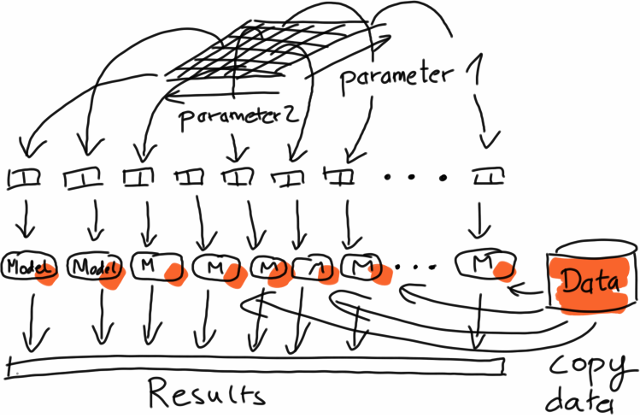
\includegraphics[scale=0.3]{images/evaluation.png}
\end{center}

(также, как и работа с признаками)

\end{frame}

% ============================================== %

\section{Особенности реальных систем}

% ============================================== %

\begin{frame}{}

\begin{center}
\Large Особенности реальных систем
\end{center}

\end{frame}

\begin{frame}{Пример обучения модели в задаче классификации}

\begin{center}
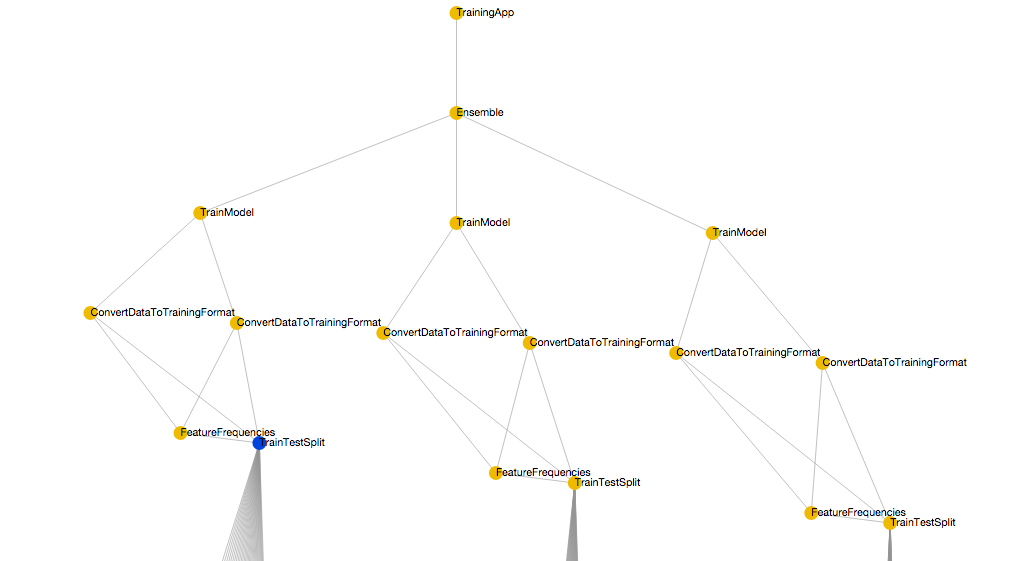
\includegraphics[scale=0.30]{images/podelie.png}
\end{center}

\end{frame}

\begin{frame}{Особенности реальной системы}

\begin{itemize}
\item Очень грязные данные
\item Простые модели
\item Проверка качества на всех этапах
\item Мониторинг и логирование
\end{itemize}

\end{frame}

% ============================================== %

\section{Что дальше}

% ============================================== %

\begin{frame}{}

\begin{center}
\Large Что дальше
\end{center}

\end{frame}

\begin{frame}{Изучение Data Mining}

\begin{enumerate}
\item Data Mining II, Hadoop, Инфопоиск
\item Kaggle
\item Литература и статьи
\begin{itemize}
\item\href{https://blog.twitter.com/engineering}{Техблог Twitter}
\item\href{http://techblog.netflix.com/?m=1}{Техблог Netflix}
\item\href{https://labs.spotify.com/}{Техблог Spotify}
\item\href{http://www.reddit.com/r/MachineLearning/}{Reddit про MachineLearning}
\item\href{http://www.thetalkingmachines.com/}{Подкаст про машинное обучение}
\item\href{http://flowingdata.com/}{DataViz}
\end{itemize}
\end{enumerate}

\end{frame}

\begin{frame}{Junior Data Scientist: необходимые навыки}

\begin{enumerate}
\item Все базовые модели и алгоритмы
\item Знание языка высокого уровня и соответствующие научные библиотеки \\ (R, python, Matlab)
\item Базовые структуры данных и алгоритмы \\ (сортировки, деревья, хэш таблицы и графы)
\item Опыт обработки больших объемов данных точно будет плюсом
\item Умение разбираться с научной литературой
\end{enumerate}

\end{frame}

\begin{frame}{}
\begin{center}

\includegraphics[scale=0.08]{images/sklearn.png}
\end{center}
\end{frame}

\begin{frame}{}

\begin{center}
\Large Вопросы
\end{center}

\end{frame}

\end{document}